\documentclass[11pt]{article}
\usepackage{amsmath}
\usepackage{comment}
\usepackage{graphicx}
\usepackage{booktabs}
\usepackage[font=small,labelfont=bf]{caption}

\begin{document}
\begin{center}
\noindent{\bf \Large{Distinguish Malignant From Benign Breast Cancer}}\vspace{1.5ex}\\
\noindent Author: Jingzhu Zhou, Xin Liu, Mengshu Shao\vspace{1.5ex}\\
\end{center}

\noindent{\bf \large{1. Introduction}} \vspace{2ex}\\
Breast cancer stage can be diagnosed by visually examining fine needle aspirate cancer cell images. The accuracy of the diagnosis is over 90\%.  However, there exists large standard error for the mean sensitivity and the mean specificity of the diagnosis. This indicates the accuracy varies greatly within individual series and visual diagnosis involves a great deal of subjectivity. 
Progress in the past 40 years in computer analysis of microscope image has made it possible for highly accurately quantitative and objective diagnosis of breast cancer. Our goal in this study is to use the computer-based analytical techniques to define the nuclear size, shape and texture, in combination with machine learning techniques to classify the eccliptical breast cells as malignant or  benign. We are expecting this method to minimize subjectivity of the visual diagnosis and increase accuracy of classification for each individual patient. \vspace{2ex}\\
The dataset which records a range of real-valued features that are computed for each cell nucleus for breast cancer diagnosis prediction. The dataset contains records of 569 instances, in which 212 are diagnosed as malignant breast cancer, and otherwise benign. The name of the dataset is “Wisconsin Diagnostic Breast Cancer” which is available on the website of UCI machine learning repository. \vspace{2ex}\\
We've considered four classification methods, which includes logistic regression, penalized logistic regression with $l1$ and $l2$ norm (namely LASSO and Ridgre regression), linear discriminant analysis, quardratic discriminant analysis and support vector machine. Before fitting a real model, we first selected the variable to keep using stepwise AIC criterion or using LASSO sparse solution. After that we did parameter variation and 10-fold cross validation, then decided with the ones with the smallest misclassification error. All the models we used can classify the breast cells into malignant or benign with an accuracy rate above 94\%. The support vector machine gave an accuracy rate as high as 97.72\%, followed by Ridge regression with a 96.49\% accuracy rate. \vspace{2ex}\\

\noindent{\bf \large{2. Methods \& Materials}} \vspace{2ex}\\
\begin{itemize}
\item {\bf\ Dataset }
\end{itemize}
The dataset we used is availabe on the website of UCI machine learning repository. Ten real-valued features are computed for each cell nucleus, including radius (mean of distances from center to points on the perimeter), texture (standard deviation of gray-scale values), perimeter, area, smoothness (local variation in radius lengths), compactness ($perimeter^2$ / area - 1.0), concavity (severity of concave portions of the contour), concave points (number of concave portions of the contour), symmetry and fractal dimension ("coastline approximation" - 1). The mean, standard error, and "worst" or largest (mean of the three
largest values) of these features were computed for each image,resulting in 30 features.  For instance, field 3 is Mean Radius, field 13 is Radius SE, field 23 is Worst Radius. The 569 patients in the dataset were either in a malignant(357) or benign(212) stage of breast cancer. They were identified by unique IDs. 
\begin{itemize}
\item {\bf Classification methods }
\end{itemize}
The classification methods we considered in this project were:\\
1) Logistic regression\\
The logistic model arises from the desire to model the probability of a binary outcome``diagnosis" via linear functions in those cell measurements. The model has the form:
\begin{center}
$logit(P(Y_i=1|X=x))=log(\frac{P(Y_i=1|X=x)}{P(Y_i\neq{1}|X=x)})=\beta_0+\beta^TX$\vspace{1.5ex}\\
\end{center}
where $Y_i=1$ denotes the diagnosis status of the individual is malignant,\\
X is a vector of predictors and $\beta$ is a vector of coefficients corresponding to those predictors.\vspace{2ex}\\
2) Penalized logistic regression\\
Considering the desire for a parsimonious and stable model, or a model which describes the response well but is as simple and stable as possible,  penalized regression allows us to accomplish the goal of subset selection, but in a more stable, continuous, and computationally efficient way. The lasso aims for parsimony using the constraint of the overall magnitude of the coefficients, thus important predictors are included in the model, and less important predictors shrink, potentially to zero. The form of the Lasso is:
\begin{center}
$\hat{\beta}^{lasso}=argmin_\beta\{\frac{1}{2}\sum_{i=1}^{n} (y_i-\beta_0-\sum_{j=1}^{p}x_{ij}\beta_j)^2+\lambda\sum_{j=1}^{p}\left|\beta_j\right|\}$\vspace{1.5ex}\\
$y_i$ are responses, $\beta_i$ are coefficients, $\lambda$ is the tuning parameter\vspace{1.5ex}\\
\end{center}
3) Linear discriminant analysis\\
Now define the linear discriminant function\\
\begin{center}
$\delta_k(x)=x^T\Sigma^{-1}\mu_k-\frac{1}{2}\mu_k^T\Sigma^{-1}\mu_k+log(\pi_k)$\\
\end{center}
Then
\begin{center}
$\hat{G}(x)=argmax_k\delta_k(x)$\\
\end{center}
The decision boundary between class $k$ and $l$ is \\
\begin{center}
${x:\delta_k(x)=\delta_l(x)}$
\end{center}
4)Quadratic discriminant analysis\\
Now define the Quadratic discriminant function
\begin{center}
$\delta_k(x)=-\frac{1}{2}log\mid \Sigma_k\mid-\frac{1}{2}(x-\mu_k)^T\Sigma_k^{-1}(x-\mu_k)+log\pi_k$\\
\end{center}
Then
\begin{center}
$\hat{G}(x)=argmax_k\delta_k(x)$
\end{center}
The decision boundary between class $k$ and $l$ is 
\begin{center}
${x:\delta_k(x)=\delta_l(x)}$
\end{center}
5)Support vector machine\\
Support Vector Machine (SVM) is primarily a classier method that performs classification tasks by constructing hyperplanes in a multidimensional space that separates cases of different class labels. To construct an optimal hyperplane, SVM employs an iterative training algorithm, which is used to minimize an error function. In our case we were trying to minimize the error function in the following form:
\begin{center}
$1/2w^Tw+C\sum_{i=1}^{N} \xi_i$,
\end{center} 
which subjects to the constraints: $y_i(w^T\phi(x_i)+b) \geq 1-\xi_i$ and $\xi_i \geq0, i = 1,...,N$. \vspace{1.5ex}\\
C is the cost constant, w is the vector of coefficients, b is a constant, and $\xi_i$ represents parameters for handling nonseparable data (inputs). The index i labels the N training cases. Note that $y_i$ represents the class labels and $x_i$ represents the independent variables. The kernel $\phi$  is used to transform data from the input (independent) to the feature space. It should be noted that the larger the C, the more the error is penalized. Thus, C should be chosen with care to avoid over fitting.
\begin{itemize}
\item{\bf Model Comparison}
\end{itemize}
The model were compared in the number of predictors and 10-fold cross validation misclassification error. The model with smaller number of predictors and a smaller misclassification error (i.e., higher accuracy) was preferable and recommended. 
\vspace{2ex}\\

\noindent{\bf \large{3. Results}} \vspace{2ex}\\
We considered penalized logistic regression, LDA \& QDA, SVM to conduct the classification. For LDA, QDA and SVM, we deleted the highly correlated variables and conducted stepwise selection to select the best subset of variables based on lowest AIC. For penalized regression, Lasso constrains the overall magnitude of the coefficients and gave out the best subset based on the lowest misclassification error. Then based on the best subset we chose, the boundary and the logistic regression model were fitted and methods were compared based on the classification error rate.
\begin{itemize}
\item {\bf\ Model Selection }
\end{itemize}
1) LDA, QDA, SVM\\
Pairwise correlations of the 30 variables were used to delete the variables that are highly correlated. Variable deleted: radius\_m,perimeter\_m,area\_w,
perimeter\_w,radius\_w,area\_sd,perimeter\_sd. \vspace{2ex}\\
Stepwise selection(logistic regression) were used to select the best subset of variables based on lowest AIC. Variable selected: concave\_points\_w, area\_m, texture\_w,radius\_sd,compactness\_sd,smoothness\_w,concavity\_w ,texture\_sd.\vspace{2ex}\\
2) Penalized Regression\\
The 10-fold cross validation chose the best tuning parameter which made the least missclassification error. The figure below plots the $log(\lambda)$ and their corresponding missclassification errors. The best tuning parameter is 0.00304, and the least missclassification error is 0.025.  \vspace{2ex}\\
The variables selected are texture\_m, concavity\_m, concave\_points\_m, fractal\_m, radius\_sd, texture\_sd, smoothness\_sd, compactness\_sd, fractal\_sd, radius\_w, texture\_w, smoothness\_w, concavity\_w, concave\_points\_w and symmetry\_w.
\begin{center}
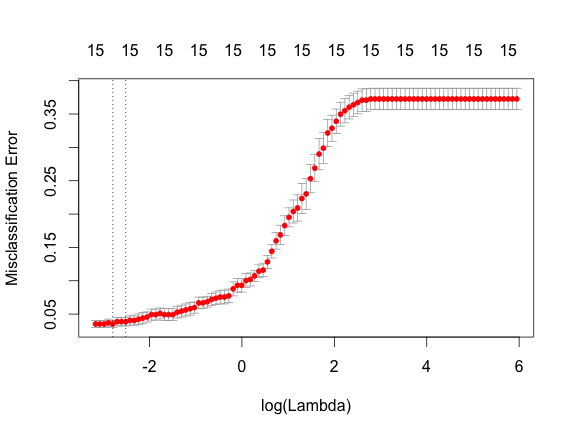
\includegraphics[width=1.0\linewidth]{Rplot}
\end{center}

\begin{itemize}
\item {\bf\ Classification }
\end{itemize}
1) SVM\\
In another set of experiments we studied the dependence of the training error found by the SVM algorithm on the parameter C. Table 2 shows the variation of the training error corresponds with the parameter C. It can be seen that the smallest error is obtained for C=0.9.
\begin{center}
\begin{tabular}{l l l l l l l l l l l} 
\toprule
\textbf{Cost} & \textbf{0.1} & \textbf{0.2} & \textbf{0.3} & \textbf{0.4} & \textbf{0.5} & \textbf{0.6} & \textbf{0.7} & \textbf{0.8} & \textbf{0.9} & \textbf{1.0}\\
\midrule
\textbf{Accuracy} & 93.85 & 95.08 & 96.31 & 96.49 & 96.84 & 97.19 & 97.19 & 97.54 & 97.72 & 97.36 \\
\bottomrule
\end{tabular}
\captionof{table}{Parameter selection for SVM}
\end{center}
2) Ridge regression\\
The best tuning parameter:0.00304. Then Ridge regression was used to fit the model based on the tuning parameter. 


$logit(P(Y_i=1|X=x))= -9.35+0.073texture_m+4.74concavity_m+14.72concave_points_m-39.34fractal_m+1.81radius_sd-0.13texture_sd-8.03smoothness_sd-2.52compactness_sd-56.07fractal_sd+0.15radius_w +0.06texture_w+12.44smoothness_w +1.58concavity_w+8.59concave_points_w+4.41symmetry_w$.


\begin{itemize}
\item {\bf\ Model Comparison }
\end{itemize}
The table below summarizes the methods, the number of parameters of each method and its corresponding accuracy.
\begin{center}
\begin{tabular}{l l l l l l} 
\toprule
\textbf{Model} & \textbf{Logistic} & \textbf{Ridge} & \textbf{LDA} & \textbf{QDA} & \textbf{SVM}\\
\midrule
Accuracy & 96.14 & 96.49 & 95.96 & 94.91 & 97.72\\
Predictor numbers & 8 & 15 & 8 & 8 &24 \\
\bottomrule
\end{tabular}
\captionof{table}{Model Comparison}
\end{center}
According to the table, all the methods gave an accuracy rate above 95\%. SVM gave the highest accuracy; however, the number of parameters is the highest. Penalized logistic regression gave the second highest accuracy, but it also used more parameters than other methods. Logistic regression gave about 96\% accuracy and only 8 parameters were chosen. LDA and QDA both chose 8 predictors and accuracy rates are lower but still around 95\%.\vspace{2ex}\\

\noindent{\bf \large{4. Discussion}} \vspace{2ex}\\ 
Given that the accuracy is consistently high for all learning algorithm, the simplicity of the model becomes important. Logistic regression, LDA and QDA used a stepwise pre-classification variable selection method that yielded 8 predictors, the smallest subset. Ridge regression,however, did not employ stepwise method but a Lasso penalized regression to shrink unimportant predictors. Support vector machine directly used the 24 predictors after the deletion of the correlated variables.  The stepwise selection is a form of hard "thresholding" whereas Lasso regression is a form of soft thresholding". Lasso regression selection is more conservative than stepwise selection(entry alpha=0.05 and elimination alpha=0.1). The subset selected by logistic regression is more preferable since the size is the smallest, given that no obvious loss in accuracy exists.   \vspace{2ex}\\ 
For classification method, the assumption of logistic regression is linearity between log odds and the predictors. On the other hand, the assumption of LDA is predictors from both classes follow a multivariate normal distribution with equal covariance structure across classes. QDA maintains the normality assumption but drops the equal covariance assumption. Support vector machine is a non-parametric method that does not have any assumptions.  \vspace{2ex}\\ 
Table.2 shows that support vector machine method has the highest accuracy rate. However, it is hard to judge whether SVM is a better performing algorithm since it used more parameters(more information) than the other methods but with only a very small improvement in accuracy.In the future, pre-classification model selection should be coupled with support vector machine in order to achieve a better comparison among models. Ridge regression has the second highest accuracy but the second highest number of predictors. Among the methods that used the 8 variable subset, logistic regression performed slightly better than LDA and QDA.  \vspace{2ex}\\ 
In the future, these models could be tested on testing dataset to calculate overall classification correction rate, sensitivity and specificity. Bootstrap could be used to build confidence intervals on these three parameters. \vspace{2ex}\\

\noindent{\bf \large{5. Conclusion}} \vspace{2ex}\\ 
In conclusion, logistic regression yielded comparably high accuracy with the  least number of predictors. Logistic regression requires the assumption of linearity. Validating the models with testing dataset and formal statistical test to compare the results should be used in the future to reach a more conclusive decision about which learning algorithm is better. \vspace{2ex}\\

\noindent{\bf \large{6. Reference}} \vspace{2ex}\\ 
\noindent1. Wolberg, William H., et al. "Computer-derived nuclear features distinguish malignant from benign breast cytology." \emph {Human Pathology} 26.7 (1995): 792-796.\vspace{1.5ex}\\
2. Wolberg, William H., et al. "Computerized breast cancer diagnosis and prognosis from fine-needle aspirates." \emph{Archives of Surgery} 130.5 (1995): 511-516.\vspace{1.5ex}\\
3. Wolberg, William H., W. Nick Street, and Olvi L. Mangasarian. "Image analysis and machine learning applied to breast cancer diagnosis and prognosis." \emph{Analytical and Quantitative cytology and histology} 17.2 (1995): 77-87.\vspace{1.5ex}



\end{document}

